\documentclass[12pt,notitlepage]{article}
\usepackage[utf8]{inputenc}
\usepackage[polish]{babel}
\usepackage[T1]{fontenc}
\usepackage{polski}
\usepackage{graphicx}
\usepackage[top=2cm, bottom=2cm, left=3cm, right=3cm]{geometry}
%\usepackage{listings}

\usepackage{xcolor}
\usepackage{lmodern}
\usepackage{listings}

\lstset{
  literate={ą}{{\k a}}1
  		     {Ą}{{\k A}}1
           {ż}{{\. z}}1
           {Ż}{{\. Z}}1
           {ź}{{\' z}}1
           {Ź}{{\' Z}}1
           {ć}{{\' c}}1
           {Ć}{{\' C}}1
           {ę}{{\k e}}1
           {Ę}{{\k E}}1
           {ó}{{\' o}}1
           {Ó}{{\' O}}1
           {ń}{{\' n}}1
           {Ń}{{\' N}}1
           {ś}{{\' s}}1
           {Ś}{{\' S}}1
           {ł}{{\l}}1
           {Ł}{{\L}}1
}

\definecolor{mGreen}{rgb}{0,0.6,0}
\definecolor{mGray}{rgb}{0.5,0.5,0.5}
\definecolor{mPurple}{rgb}{0.58,0,0.82}
\definecolor{backgroundColour}{rgb}{0.95,0.95,0.92}

\lstdefinestyle{CStyle}{
    backgroundcolor=\color{backgroundColour},   
    commentstyle=\color{mGreen},
    keywordstyle=\color{magenta},
    numberstyle=\tiny\color{mGray},
    stringstyle=\color{mPurple},
    basicstyle=\footnotesize,
    breakatwhitespace=false,         
    breaklines=true,                 
    captionpos=b,                    
    keepspaces=true,                 
    numbers=left,                    
    numbersep=5pt,                  
    showspaces=false,                
    showstringspaces=false,
    showtabs=false,                  
    tabsize=2,
    language=C
}


\makeatletter

\newcommand{\linia}{\rule{\linewidth}{0.4mm}}

\renewcommand{\maketitle}{\begin{titlepage}



    \noindent\linia

    \begin{center}

      \LARGE \textsc{\@title}

         \end{center}

     \linia

    \vspace{0.5cm}
    
        \vspace*{1cm}

    \begin{center}\Large

    Grupa numer 16\\

Informatyka\\
II rok\\
Rok akademicki 2017/2018\\

    \end{center}

    \vspace{3cm}

%    \begin{flushright}

	\begin{center}
	
    \begin{minipage}{6cm}
\begin{center}

    \textit{\normalsize Autorzy:}\\

\end{center}
    \Large \textsc{\@author} \par

    \end{minipage}

	\end{center}
    \vspace{5cm}



%     \end{flushright}

    \vspace*{\stretch{6}}

    \begin{center}

    \@date

    \end{center}

  \end{titlepage}%

}

\makeatother

\author{Kolano Grzegorz\\
	Wiater Mateusz\\
	Wolski Łukasz\\
}

\title{Ping Pong}

\begin{document}

\maketitle

\newpage

\section{Użyte moduły}
\subsection{Arduino Uno}
\begin{figure}[h!]
  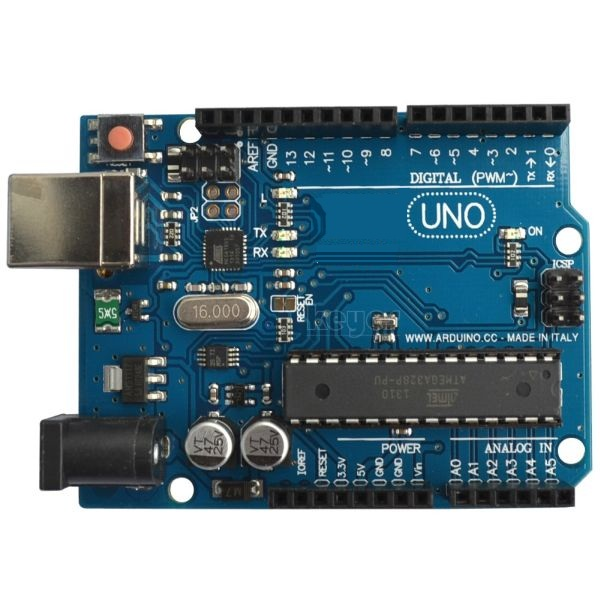
\includegraphics[width=\textwidth]{uno.jpg}
  \label{fig:uno}
\end{figure}
\newpage
\subsection{Matryca LED 8x8 ze sterownikiem MAX7219}
\begin{figure}[h!]
  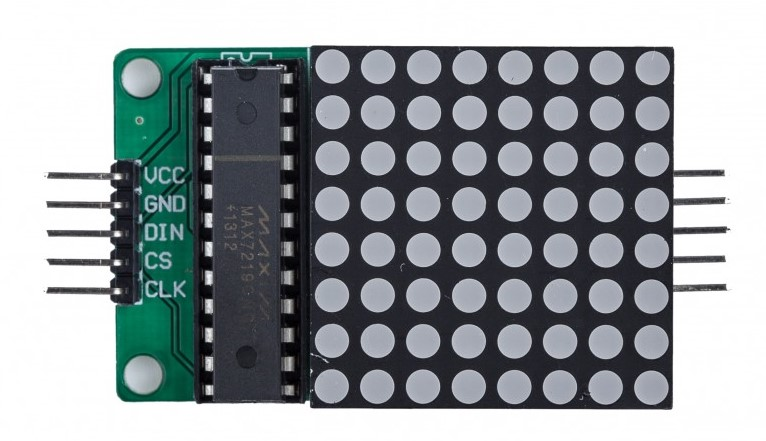
\includegraphics[width=\textwidth]{matrix.jpg}
  \label{fig:matrix}
\end{figure}

\subsection{Joystick analogowy}
\begin{figure}[h!]
  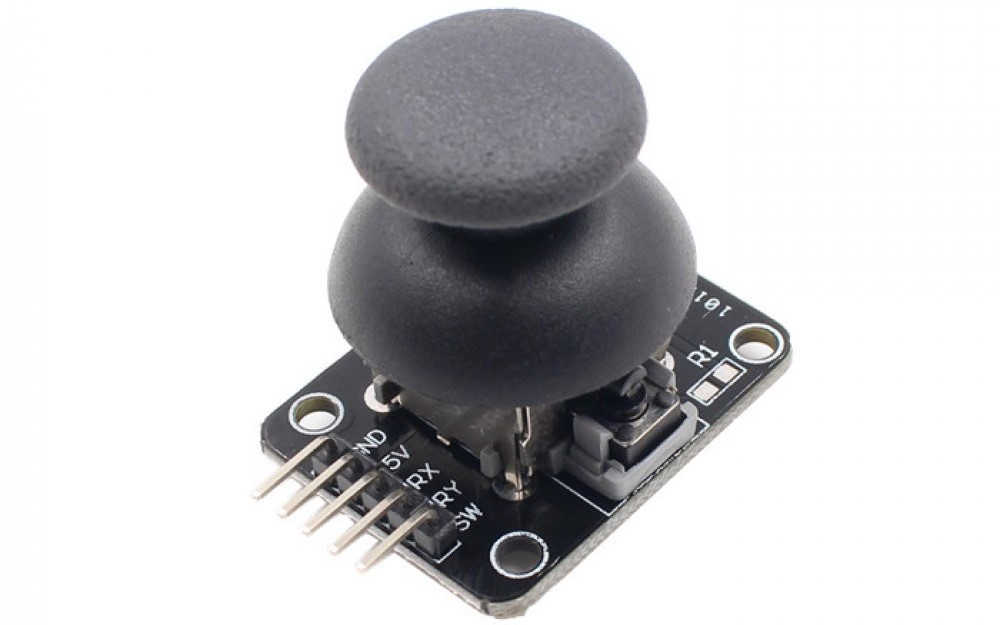
\includegraphics[width=\textwidth]{joystick.jpg}
  \center
  \label{fig:joystick}
\end{figure}
\newpage

\section{Schematy połączeń}
\subsection{Arduino-Matryca LED}
\begin{figure}[h!]
   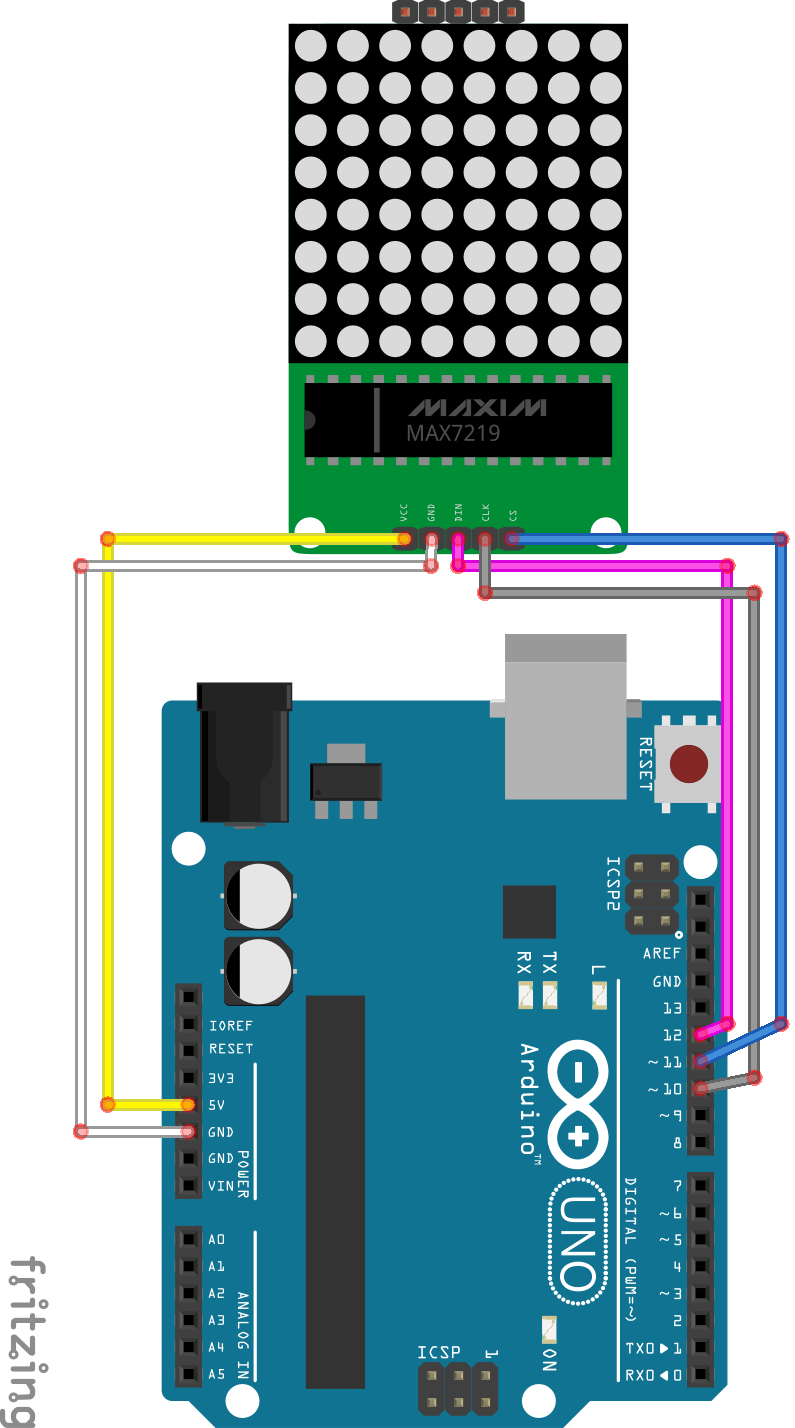
\includegraphics[height=0.9\textheight]{schemat-plytka-matryca_bb.png}
   \centering
  \label{fig:schemat-plytka-matryca}
\end{figure}

\subsection{Arduino-Joystick}
\begin{figure}[h!]
   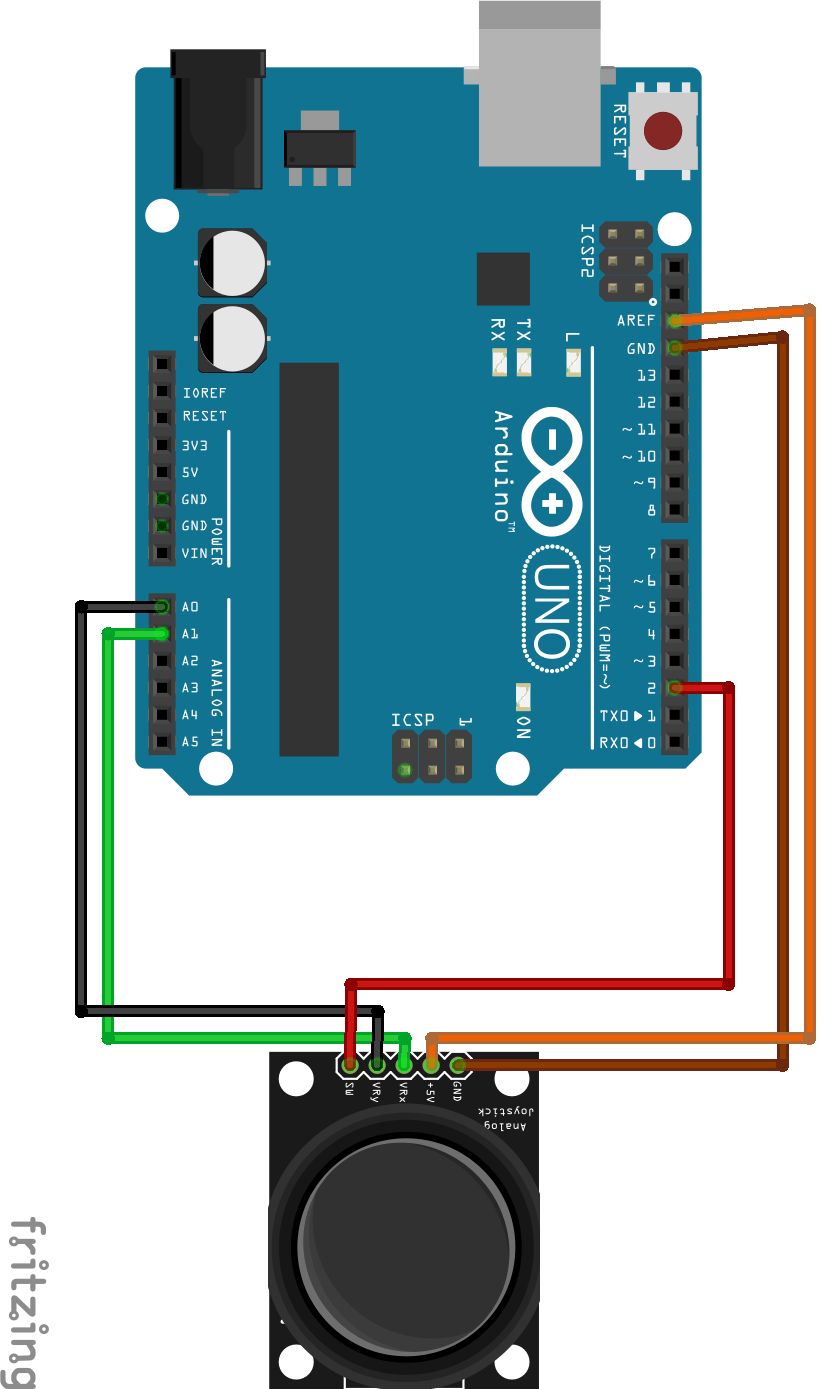
\includegraphics[height=0.9\textheight]{schemat_plytka-joystick.png}
   \centering
  \label{fig:schemat-plytka-joystick}
\end{figure}

\subsection{Całość}
\begin{figure}[h!]
   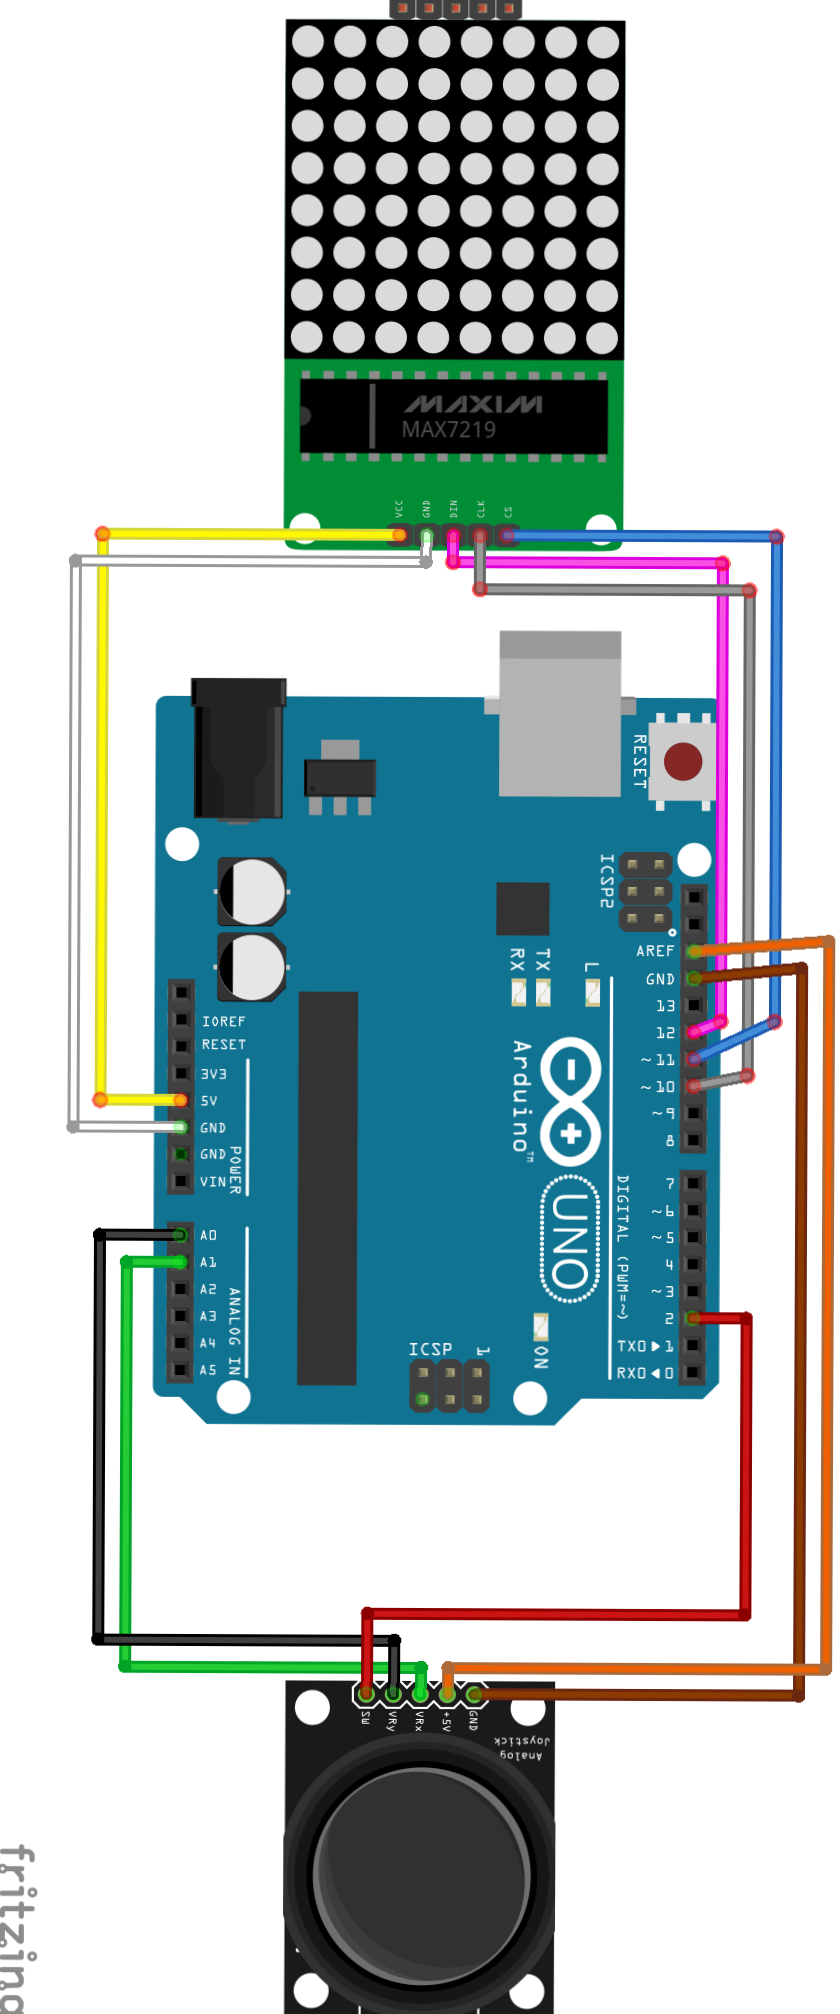
\includegraphics[height=0.9\textheight]{schemat_bb.png}
   \centering
  \label{fig:schemat-calosc}
\end{figure}

\section{Opis programu}

Gra rozpoczyna się widokiem rakietki, start nastąpi po naciśnięciu joysticka, wtedy piłeczka pojawi się losowo w jednym
z dwóch pikseli. W tym celu wykorzystano funkcję $randomSeed$ z argumentem $analogRead(A2)$, dzięki czemu funkcja random 
przy każdym uruchomieniu zwracała losową wartość, gdyż do wejścia $A2$ nie podłączono żadnego sygnału.
Na tym opiera się również losowość odbicia piłeczki od lewej krawędzi lub rakietki.

Pierwsze współrzędne pikseli rakietki są przechowywane w tablicy $bat$, a współrzędne piłeczki przechowują zmienne $r\_ball$ i $c\_ball$.
W trakcie gry funkcja $points$ sprawdza czy piłeczka pokryła się z rakietką i na tej podstawie są przyznawane punkty, które przechowuje zmienna $score1$.
Punkty są wyświetlane w postaci binarnej na migającym ekranie (po przegranej) lub po naciśnięciu joysticka w trakcie gry w zerowej kolumnie.
Wraz ze zdobyciem określonej ilości punktów, zwiększa się również poziom gry (zmienna $lvl$), a razem z nim tempo $SP\_BALL$ poruszania się piłeczki.

W trakcie gry jest możliwe przyspieszanie lub zwalnianie tempa poruszania się piłeczki. Ze względu na dużą czułość joysticka, łatwo było o
przypadkową zmianę tempa. W tym celu zostało wprowadzono zabezpieczenie polegające na tym, że cały system zmiany tempa należy odblokować
przez wychylenie joysticka w jedną ze stron (tak jak przy normalnej zmianie tempa), dopiero od tej chwili będą możliwe zmiany tempa w ciągu
800ms od poprzednich zmian (wychyleń).
Tempa nie można zmienić powyżej wartości $SP\_LIMIT$ (im wyższa wartość $SP\_BALL$ tym piłeczka porusza się wolniej).
Jeśli udało nam się przyspieszyć lub zwolnić tempo piłeczki zamigają dwie diody na górze lub dole ekranu, a w przypadku niepowodzenia tylko jedna.

Jeśli josystick zostanie naciśnięty na mniej niż 1 sekudnę, w zerowej kolumnie pokażą się punkty, a w drugiej szanse.
Co każdą sekundę przytrzymania joysticka nastąpi też zmiana rozmiaru rakietki. 
W momencie naciśnięcia joysticka gra w rzeczywistości się nie zatrzymuje, a bardzo zwalnia, piłeczka będzie niewidoczna i zmieniała pozycję co 30 sekund.

Aby piłeczka, rakietka oraz pozostałe mechanizmy mogłby pracować niezależnie, pomocna okazała się funkcja $millis$ umożliwiająca wprowadzenie wielozadaniowości.
Do wyświetlania piłeczki, rakietki oraz innych elementów gry wykorzystana została funkcja $setLed$, którą zawiera biblioteka $LedControl$.
\section{Biblioteka LedControl}
Biblioteka $LedControl.h$ jest biblioteką dla sterowników MAX7221 i MAX7219, które w prosty sposób umożliwiają kontrolę nad LED-ową matrycą 8x8 pikseli.
\newpage
\section{Listing kodu źródłowego}

\begin{lstlisting}[style=CStyle]

int RSIZE=1; // rozmiar paletki
int POINTS=3; // liczba żyć

int R = 0; int C = 0; //położenie joysticka R (row) i C (column)

int r_translate = 4; int c_translate = 7; // główny punkt rakietki (wszystkie inne są wyświetlane na podstawie tego, jesli ustawimy RSIZE=1 to rakietka wyswietli sie dokladnie w tym miejscu
int r_old = 4; // sluzy do czyszczenia starego polozenia rakietki (stary wiersz), zmienna c_old nie jest potrzebna, bo rakietka zawsze jest w 7 kolumnie

int c_ball = 0; //poczatkowo pileczka znajduje sie w 0 kolumnie
int r_ball; 
int R_ball=1; // Przy rozpoczeciu gry, wiersz w ktorym pojowia sie pileczka jest losowy, ta zmiena kontroluje czy gra zostala wczytana poraz pierwszy 
int br_old; int bc_old=0; //sluza do czyszczenia starego polozenia pileczki ball row/column
int lr=2; //=1 pileczka porusza sie w lewo, =2 pileczka porusza sie w prawo

int SP_BALL=400; //predkosc pileczki, w tej chwili pileczka bedzie zmieniala polozenie co 400ms
int sp_controller1=1;int sp_controller2=0; //pomocnicze zmienne, które zostaly wykorzystane do zabezpieczenia zmiany szybkosci pileczki, aby nie zmieniac jej przez przypadek w trakcie gry
unsigned long spch_timer = 0; //zmienna pomocnicza do zmiany tempa pileczki, speed change
int led_sp=0; unsigned long led_sp_t=0; //gdy uda nam sie zmienic tempo zaswieca sie dwie diody (na gorze lub nadole w zaleznosci od tego czy przyspieszamy czy zwalniamy)


int vec; // wykorzystane do tego aby pileczka poruszala sie w losowym kierunku
unsigned long now = 0; // https://forbot.pl/blog/kurs-arduino-ii-wielozadaniowosc-opoznienia-z-millis-id18418
unsigned long last = 0; //wykorzystane do szybkosci przesuwania sie rakietki
unsigned long b_last = 0; //wykorzystane do szybkosci przesuwania sie pileczki
int bat[] = {-6,-6,-6,-6,-6}; // -6 ponieważ rakietka o rozmiarze 5 moze sie calkowicie znalezc poza planszą i jeden punkt by mial wartosc -5 (lub 5)

//Poziomy
int lvl=1; int score1=0; //aktualny lv i punkty
int SP_LIMIT=400; // najwolniejsze mozliwe tempo pileczki, nie bedzie sie dalo zwolnic powyzej tej wartosci

//Rozmiar rakietki
int R_SIZE; //bedzie przechowywala rozmiar pileczki, ktory moze sie rowzniez zmieniac w trakcie gry
boolean firstgame=true; // wartosc RSIZE bedzie wykorzystana tylko przy pierwszym wczytaniu gry

//SW (switch czyli wciskanie joysticka)
unsigned long sw_timer = 0; //sprawdzi czy joy jest przytrzymywany
int sw_c=0; // sluzy do zmiany rozmiaru rakietki
int SP_BALL_temp=SP_BALL; //w momencie wcisniecia joya gra bardzo zwalnia
int newgame=0; //sluzy do resetowania gry jesli przegramy

#include "LedControl.h" //  need the library
LedControl lc=LedControl(12,10,11,1); //10 is to CLOCK, 9 = CS, 8=DIN//
const int SW_pin = 2; //Switch do 2

void setup() {
  Serial.begin(57600);
  pinMode(SW_pin,INPUT);
  digitalWrite(SW_pin, HIGH);

  lc.shutdown(0,false);// turn off power saving, enables display
  lc.setIntensity(0,0);// sets brightness (0~15 possible values)
  lc.clearDisplay(0);// clear screen
  randomSeed(analogRead(A2));
}

void loop() {
  if(firstgame)R_SIZE=RSIZE;
  if(POINTS>0){
        //general
        firstgame=false;
        now = millis();
        if(R_ball){r_ball = random(3,5); R_ball=0; br_old=r_ball;}      
      
        //rakietka
        if(now - last >= 105){
          last = now;
          //czyszczenie rakietki
         lc.setLed(0,r_old,c_translate,false);
         if(R_SIZE>=2)lc.setLed(0,r_old-1,c_translate,false);
         if(R_SIZE>=3)lc.setLed(0,r_old+1,c_translate,false);
         if(R_SIZE>=4)lc.setLed(0,r_old-2,c_translate,false);
         if(R_SIZE==5)lc.setLed(0,r_old+2,c_translate,false);
          
          //Wyświetlanie i ruchy paletką
          lc.setLed(0,r_translate,c_translate,true);
          if(R_SIZE>=2)lc.setLed(0,r_translate-1,c_translate,true);
          if(R_SIZE>=3)lc.setLed(0,r_translate+1,c_translate,true); 
          if(R_SIZE>=4)lc.setLed(0,r_translate-2,c_translate,true);
          if(R_SIZE==5)lc.setLed(0,r_translate+2,c_translate,true);
          
          if(R_SIZE>=4)bat[0]=r_translate-2;
          if(R_SIZE>=2)bat[1]=r_translate-1;
          bat[2]=r_translate;
          if(R_SIZE>=3)bat[3]=r_translate+1;
          if(R_SIZE==5)bat[4]=r_translate+2;
          R = analogRead(A1);
          int r_temp = map(R, 1023, 0, 7, 0);
          r_old=r_translate; //do wyczyszczenia starego polozenia
           
          //wartosci dla nowego położenia rakietki
          if(r_translate<7+R_SIZE and r_translate>0-R_SIZE){
            if(r_temp>5) r_translate++; else if(r_temp<3) r_translate--;
          }
          else if(r_translate<=0){ if(r_temp>5) r_translate++;}
          else {if(r_temp<3) r_translate--;}
         }
          if(newgame==0 and digitalRead(SW_pin)==HIGH)newgame=1;
          if(newgame==1 and digitalRead(SW_pin)==LOW)newgame=2;
          if(newgame==2){
         //piłeczka
         if(now - b_last >= SP_BALL){
          b_last=now;
          lc.setLed(0, br_old, bc_old, false);
          
         //rysowanie piłeczki
          lc.setLed(0, r_ball, c_ball, true);          
          br_old=r_ball; bc_old=c_ball;
          //punkty
          if(c_ball==7) {
            if(points(r_ball, bat)==1){score1++;}
            else{
              POINTS-=1;
              showPoints(POINTS);
              showScore(score1);
              delay(700);
              lc.clearDisplay(0);
            }
          }          
          //wartość r dla nowego położenia piłeczki
	if(c_ball==0 and r_ball<=6 and r_ball>=1 and c_ball!=7){		  
              vec=random(-1,2);
              r_ball=vec+r_ball;
          }
          else if(r_ball==0){
            r_ball++;
            vec=1;
          }
          else if(r_ball==7){
            r_ball--;
            vec=-1;
          }
          else if(c_ball==7){
            switch(random(0,5)){
              case 0:
                r_ball++;
                break;
               case 1:
                r_ball--;
                break;
               case 2:
                break;
               default:
                r_ball=r_ball+vec; 
            }
          }
          else{
            r_ball=vec+r_ball;
          }
          //wartość c dla nowego położenia piłeczki
          if(lr==2)c_ball++;
          if(lr==1)c_ball--;
          if(c_ball==0)lr=2;
          if(c_ball==7)lr=1;
         }
         //Zmiana szybkości piłeczki
          C = analogRead(A0);
          int c_temp = map(C, 1023, 0, 0, 255);
          int r_temp = map(R, 1023, 0, 255, 0);
          
          if((c_temp==255 or c_temp==0) and r_temp==132 and sp_controller1==1){sp_controller2=1; sp_controller1=0; spch_timer=now;}
          if(c_temp==127 and r_temp== 132 and sp_controller2==1){sp_controller1=2;}
          if((now-spch_timer>=50 and now-spch_timer<=800) and sp_controller2==1 and sp_controller1==2){
            //ZWOLNIENIE    
            if(c_temp==255 and r_temp== 132){
              sp_controller2=0; sp_controller1=1;
              if(SP_BALL<=SP_LIMIT-25){
                SP_BALL+=25;  
                lc.setLed(0,7,3,true); lc.setLed(0,7,4,true); led_sp=1; led_sp_t=now ;
              }else{
                SP_BALL=SP_LIMIT;  
                lc.setLed(0,7,3,true); led_sp=1; led_sp_t=now ;          
              }
            }
            //PRZYSPIESZENIE
            else if(c_temp==0 and r_temp== 132){
              sp_controller2=0; sp_controller1=1;
              if(lvl<5){
                SP_BALL-=25;
                lc.setLed(0,0,3,true); lc.setLed(0,0,4,true); led_sp=1; led_sp_t=now ;
              }else{
                SP_BALL=SP_LIMIT;  
                lc.setLed(0,0,3,true); led_sp=1; led_sp_t=now ;
              }
            }      
          }
          //gaszenie ledów
          if(led_sp==1 and now-led_sp_t>100){
            led_sp=0;
            lc.setLed(0,7,3,false); lc.setLed(0,7,4,false);
            lc.setLed(0,0,3,false); lc.setLed(0,0,4,false);
          }
          //blokada zmiany tempa
          else if(now-spch_timer>800){sp_controller1=1; sp_controller2=0;}          
      
          //POZIOMY
          if(score1==4){SP_LIMIT=360; if(SP_BALL>360)SP_BALL=360;lvl=2;}
          if(score1==10){SP_LIMIT=320; if(SP_BALL>320)SP_BALL=320; lvl=3;}
          if(score1==20){SP_LIMIT=290; if(SP_BALL>290)SP_BALL=290;lvl=4;}
          if(score1==30){SP_LIMIT=260; if(SP_BALL>260)SP_BALL=260;lvl=5;}
          if(score1==40){SP_LIMIT=240; if(SP_BALL>240)SP_BALL=240;lvl=6;}
          if(score1==50){SP_LIMIT=220; if(SP_BALL>220)SP_BALL=220;lvl=7;}
          if(score1==60){SP_LIMIT=200; if(SP_BALL>200)SP_BALL=200;lvl=8;}
                
          //Zmiana rozmiaru
          if(digitalRead(SW_pin)==LOW){
            if(sw_c==0){
              sw_c=1;
              SP_BALL_temp=SP_BALL;
              SP_BALL=30000;
              lc.setLed(0,br_old,bc_old,false);
            }
            showScore(score1);
            showPoints(POINTS);
            if(sw_c==1){sw_timer=now;sw_c=2;}
            if(now-sw_timer>1000 and sw_c==2){
              sw_c=1;
              for(int i=0; i<=7;i++){
                lc.setLed(0,i,7,false);
              }
              if(R_SIZE==5){
                R_SIZE=1;
                bat[0]=-6;bat[1]=-6;bat[3]=-6;bat[4]=-6;
              }
              else  R_SIZE++;
            }
          }          
          if(digitalRead(SW_pin)==HIGH and sw_c>=1){
              for(int i=0; i<=7;i++){
                lc.setLed(0,i,0,false);
              }
              for(int i=0; i<=7;i++){
                lc.setLed(0,i,2,false);
              }
              sw_c=0;
              SP_BALL=SP_BALL_temp;
          }
      }
     
  }else if(POINTS==0){lc.clearDisplay(0);POINTS=-1; newgame=0;}
  else{
    now=millis();
    
    if(now-sw_timer<1500)showScore(score1);
    else if(now-sw_timer==1500) lc.clearDisplay(0);
    else if(now-sw_timer>=1650) sw_timer=now;
    if(digitalRead(SW_pin)==LOW){R = 0;lc.clearDisplay(0);
        C = 0;
        r_translate = 4;
        c_translate = 7;
        r_old = 4;bc_old=0;
        c_ball = 0;lr=2;
        SP_BALL=400; sp_controller1=1;sp_controller2=0;spch_timer = 0;
        led_sp=0;led_sp_t=0;
        R_ball=1;
        now = 0;
        last = 0;
        b_last = 0;
        bat[0]=-6; bat[1]=-6;bat[2]=-6;bat[3]=-6;bat[4]=-6;
        //Poziomy
        lvl=1;score1=0;
        SP_LIMIT=400;
        POINTS=3;
        sw_timer = 0;
        sw_c=0;
        SP_BALL_temp=SP_BALL;
        newgame=0;
      }
  }   
}

//FUNKCJE
int points(int _r, int _bat[]){
  for(int i=0; i<5; i++){
    if(_r==_bat[i]) return 1;
  }
  return 0;
}

int showPoints(int _points){
  int i=7;
  for(; _points>0; _points--){
    lc.setLed(0,7-i,2,true);
    i--;
  }
}

int showScore(int value){
  int tab[8]={0,0,0,0,0,0,0,0};
  for(int i=7; i>=0; i--){
    if(value%2==1){
      tab[i]=1;
      value=(value-1)/2;
    }
    else{
      tab[i]=0;
      value=value/2;
    }
  }
  for(int i=0; i<=7;i++){
    if(tab[i]) lc.setLed(0,7-i,0,true);
  }
}
\end{lstlisting}

\end{document}